% Chương 4 

\chapter{DEMO VÀ ĐÁNH GIÁ PHƯƠNG PHÁP} 

\label{Chapter4}

\section{Demo sản phẩm}



\subsection{Sử dụng công cụ MediaPipe và xây dựng mạng LSTM}
\begin{itemize}
    \item Swing
    
        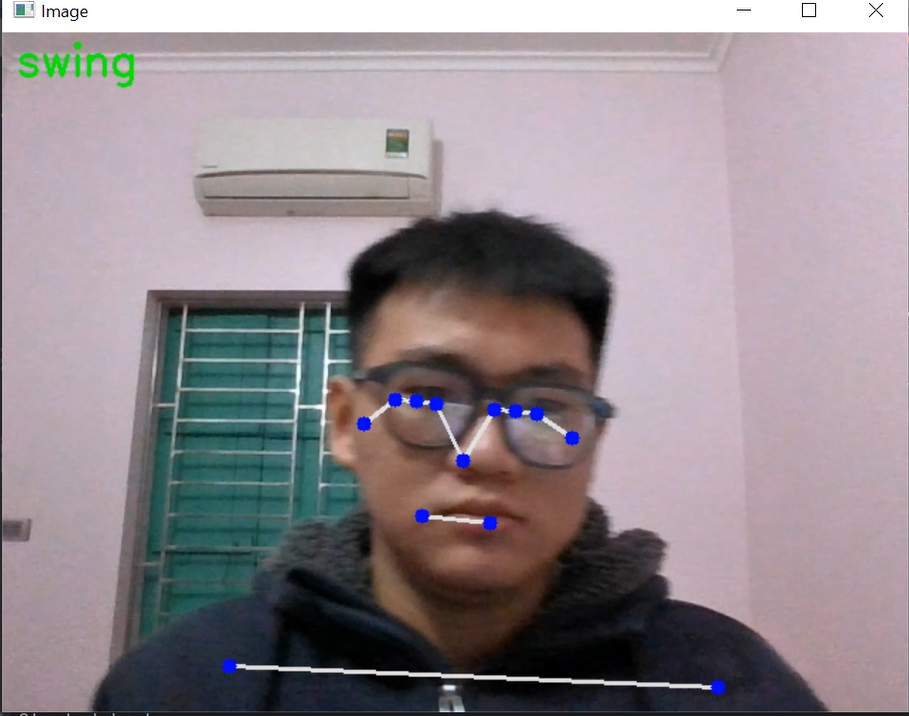
\includegraphics[width=0.5\textwidth]{Figures/swing.PNG}
        \begin{figure}[h!]
    	\centering
    	\caption[Swing output .]{Swing output.}
    	\label{bia_conv.png} 
        \end{figure}
    \item Hand Swing

        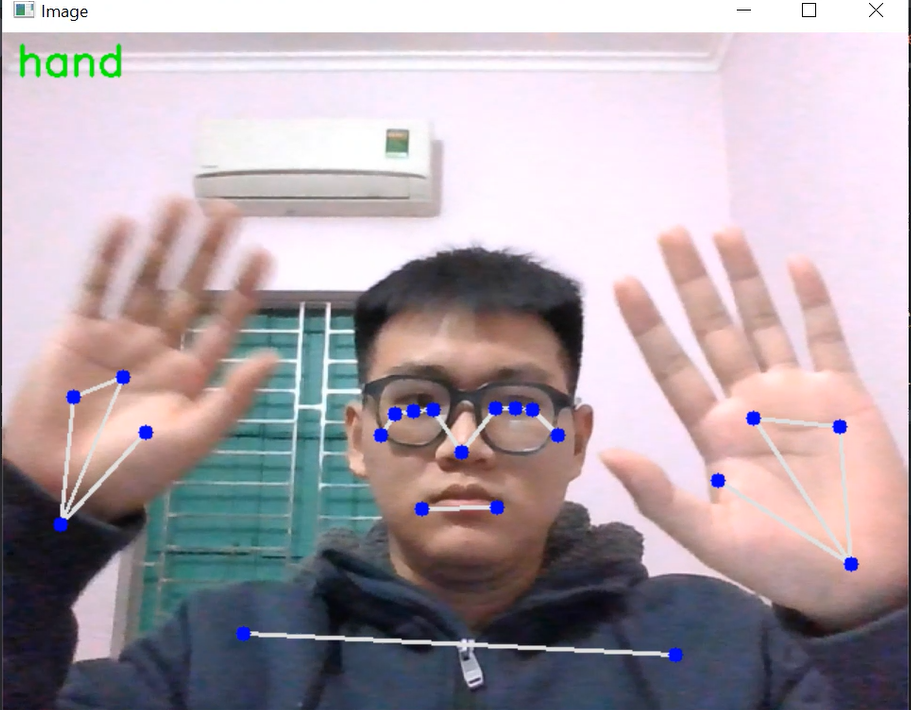
\includegraphics[width=0.5\textwidth]{Figures/hand.PNG}
        \begin{figure}[h!]
    	\centering
    	
    	\caption[Hand Swing output .]{Hand Swing output.}
    	\label{hand.png} 
        \end{figure}
    \item Love

        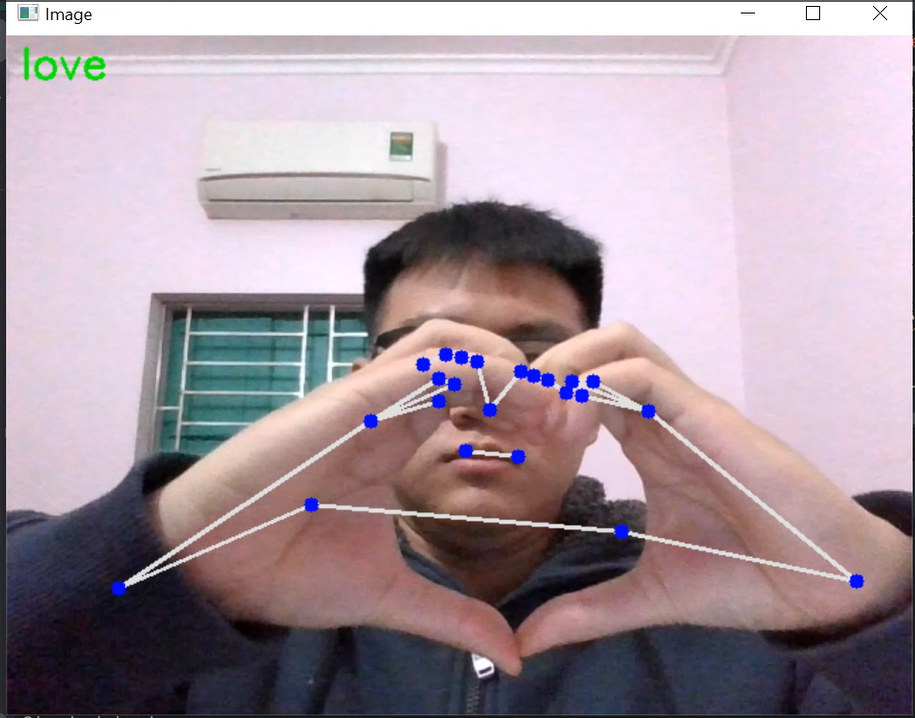
\includegraphics[width=0.5\textwidth]{Figures/love.PNG}
        \begin{figure}[h!]
    	\centering
    	
    	\caption[Love output .]{Love output.}
    	\label{love.png} 
        \end{figure}
        
    \item Clap

        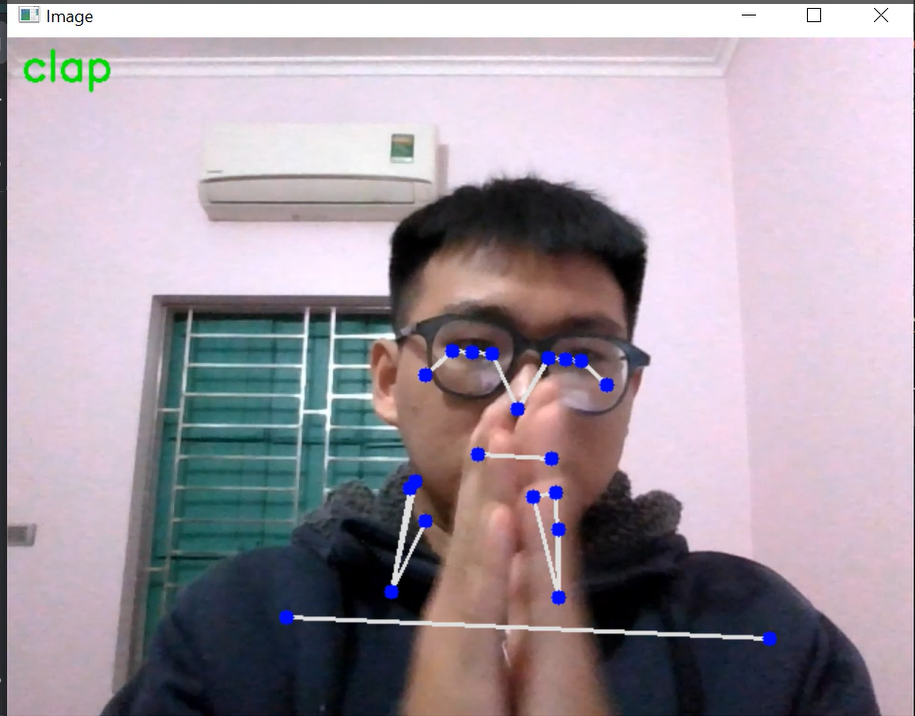
\includegraphics[width=0.5\textwidth]{Figures/clap.PNG}
        \begin{figure}[h!]
    	\centering
    	
    	\caption[Clap output .]{Clap output.}
    	\label{clap.png} 
        \end{figure}

    \item Doze

        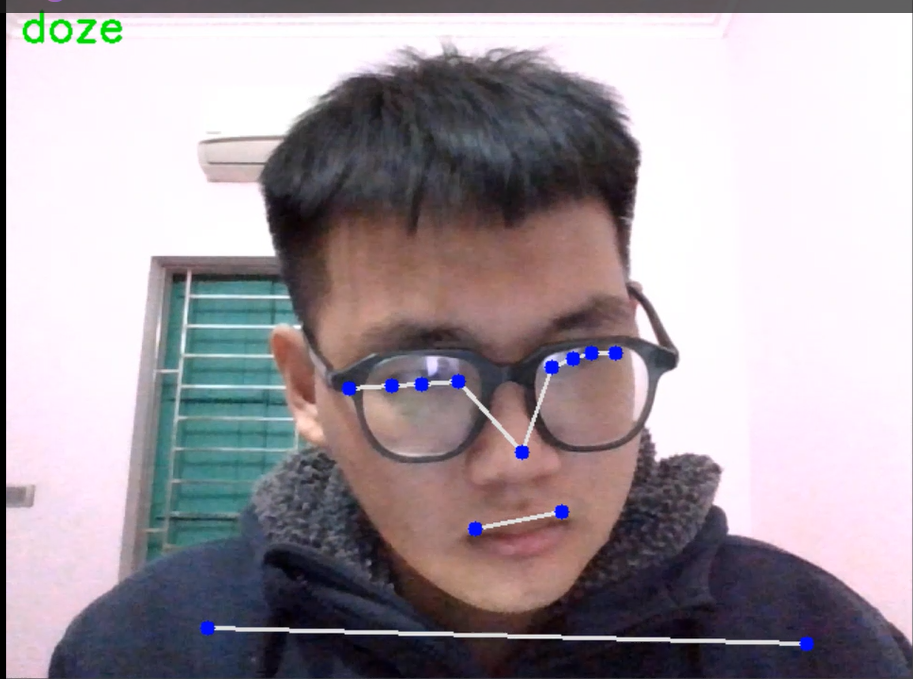
\includegraphics[width=0.5\textwidth]{Figures/doze.PNG}
        \begin{figure}[h!]
    	\centering
    	
    	\caption[Doze output .]{Doze output.}
    	\label{doze.png} 
        \end{figure}
\end{itemize}

\subsection{Mô hình ConvLSTM}
\begin{itemize}
    \item Billards
    
        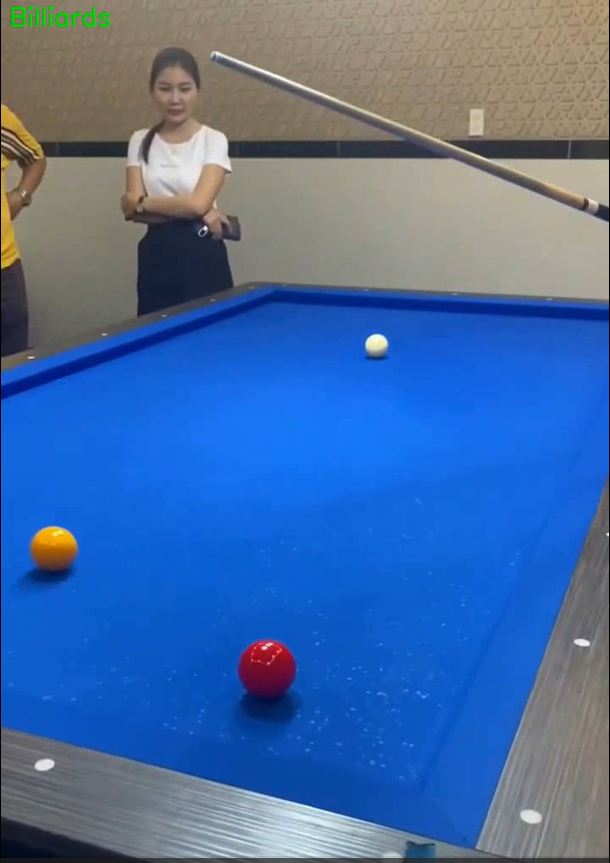
\includegraphics[width=0.5\textwidth]{Figures/bia_conv.png}
        \begin{figure}[h!]
    	\centering
    	\caption[Billards output .]{Billards output.}
    	\label{bia_conv.png} 
        \end{figure}
    \item Soccer Juggling

        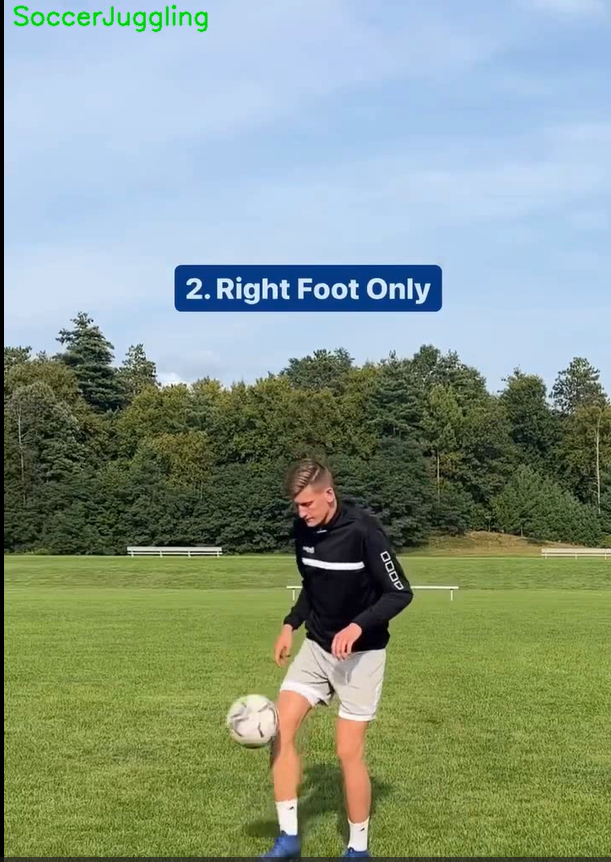
\includegraphics[width=0.5\textwidth]{Figures/soccer_conv.png}
        \begin{figure}[h!]
    	\centering
    	
    	\caption[Soccer Juggling output .]{Soccer Juggling output.}
    	\label{soccer_conv.png} 
        \end{figure}
    \item Swing

        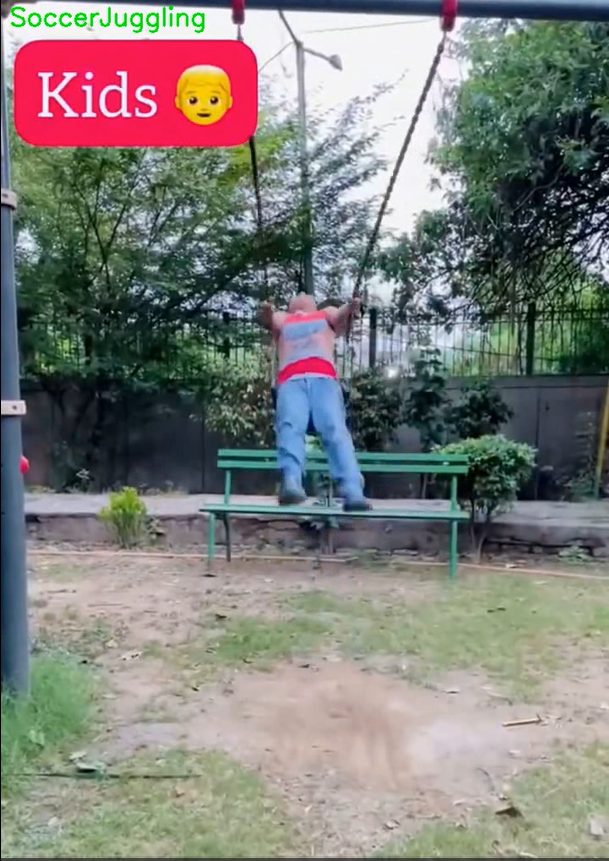
\includegraphics[width=0.5\textwidth]{Figures/swing_conv.png}
        \begin{figure}[h!]
    	\centering
    	
    	\caption[Swing output .]{Swing output.}
    	\label{swing_conv.png} 
        \end{figure}
        
    \item HorseRace

        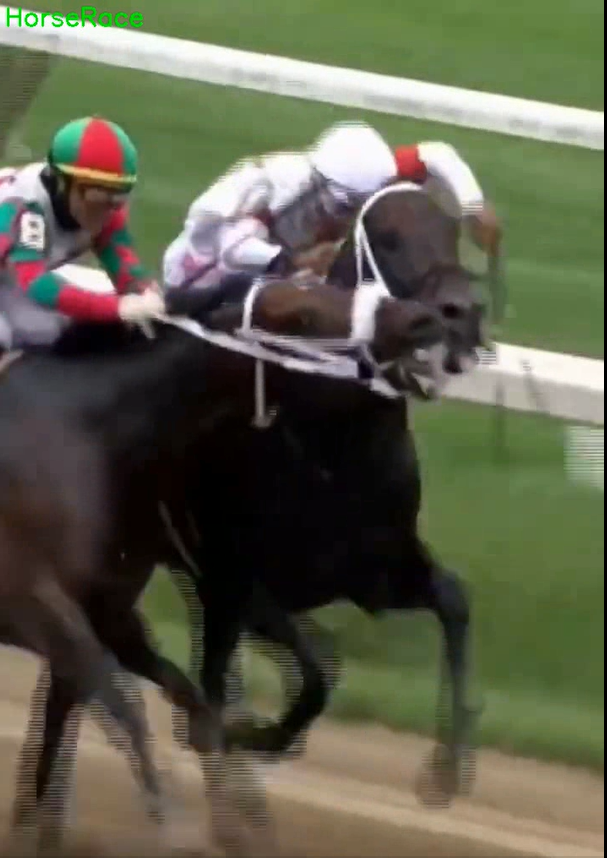
\includegraphics[width=0.5\textwidth]{Figures/race_conv.png}
        \begin{figure}[h!]
    	\centering
    	
    	\caption[HorseRace output .]{HorseRace output.}
    	\label{race_conv.png} 
        \end{figure}

    \item PlayingPiano

        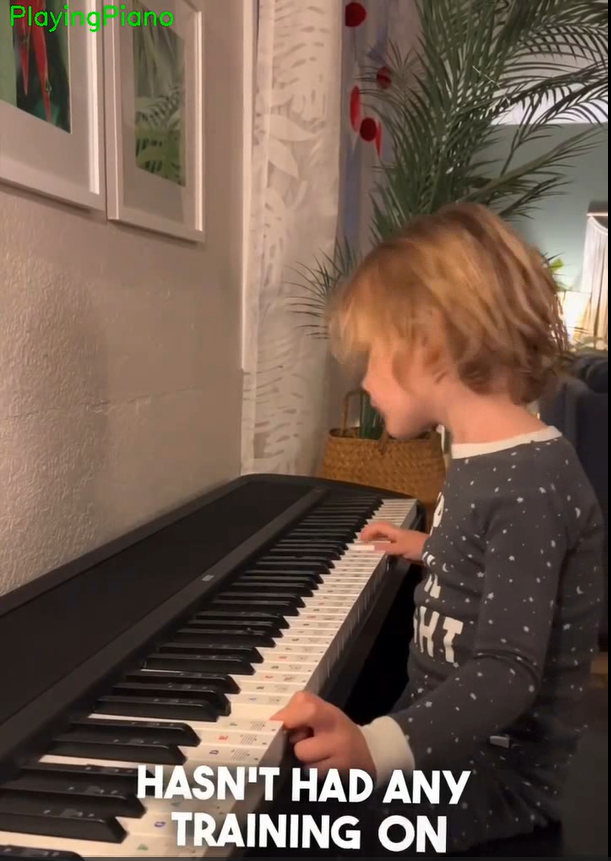
\includegraphics[width=0.5\textwidth]{Figures/piano_conv.png}
        \begin{figure}[h!]
    	\centering
    	
    	\caption[PlayingPiano output .]{PlayingPiano output.}
    	\label{piano_conv.png} 
        \end{figure}

    \item PushUps

        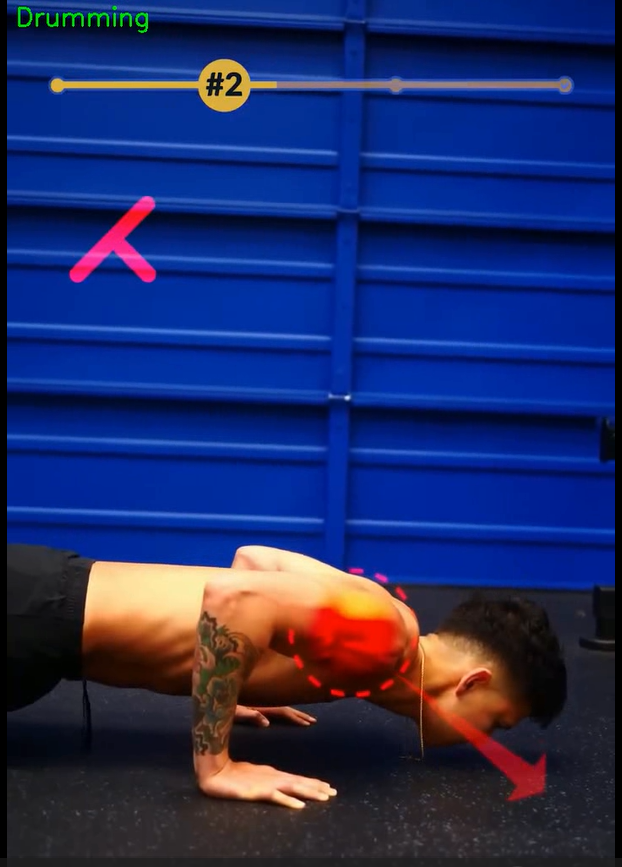
\includegraphics[width=0.5\textwidth]{Figures/pushup_conv.png}
        \begin{figure}[h!]
    	\centering
    	
    	\caption[PushUps output .]{PushUps output.}
    	\label{pushup_conv.png} 
        \end{figure}
        
    \item Skijet

        
\includegraphics[width=0.5\textwidth]{Figures/skijet_conv.png}
        \begin{figure}[h!]
    	\centering
    	
    	\caption[Skijet output .]{Skijet output.}
    	\label{skijet_conv.png} 
        \end{figure}

    \item Drumming

        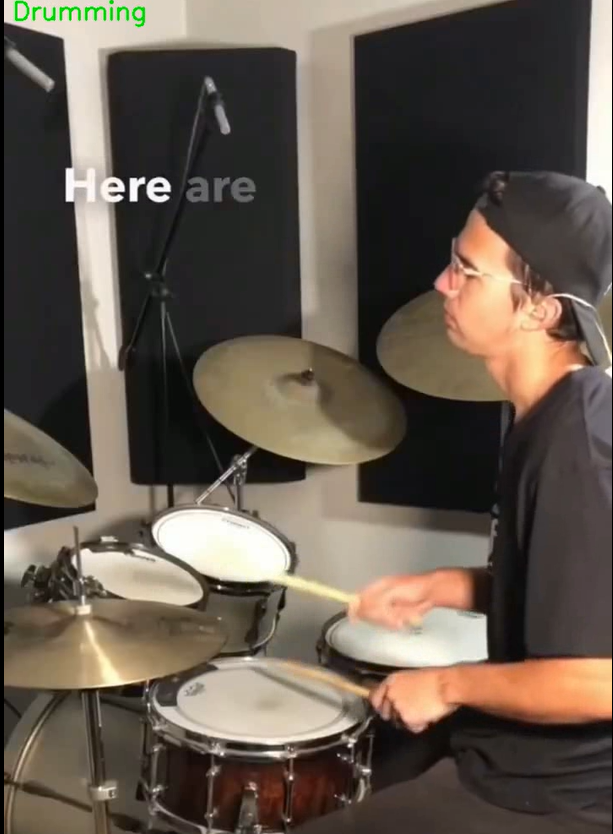
\includegraphics[width=0.5\textwidth]{Figures/drum_conv.png}
        \begin{figure}[h!]
    	\centering
    	
    	\caption[Drumming output .]{Drumming output.}
    	\label{drum_conv.png} 
        \end{figure}
    
\end{itemize}
    


\subsection{Mô hình LRCN}

\begin{itemize}
    \item Billards
    
        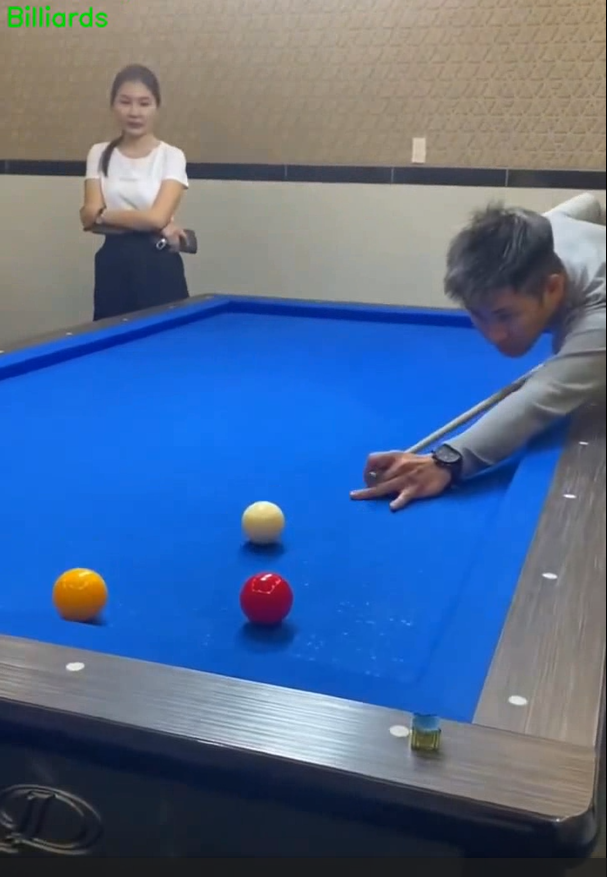
\includegraphics[width=0.5\textwidth]{Figures/bia_lrcn.png}
        \begin{figure}[h!]
    	\centering
    	\caption[Billards output .]{Billards output.}
    	\label{bia_lrcn.png} 
        \end{figure}
    \item Soccer Juggling

        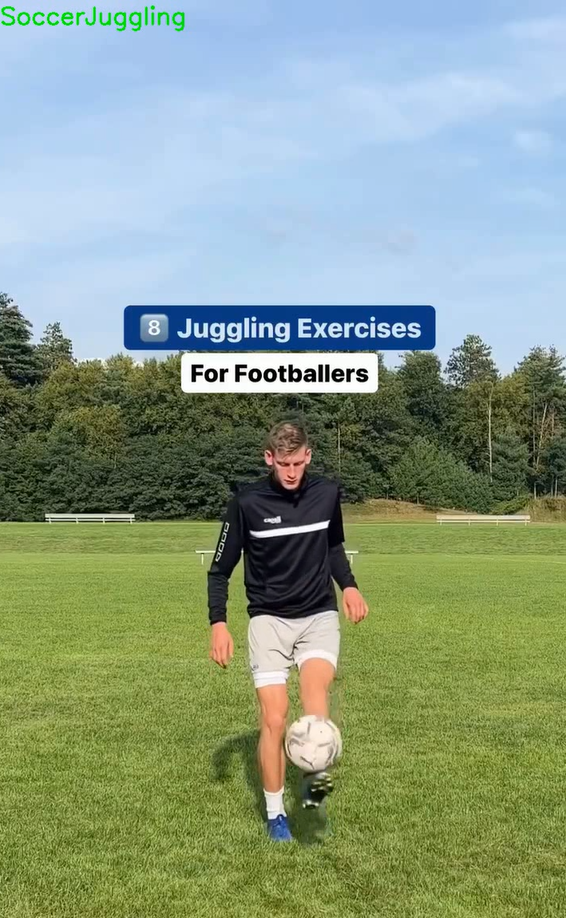
\includegraphics[width=0.5\textwidth]{Figures/soccer_lrcn.png}
        \begin{figure}[h!]
    	\centering
    	
    	\caption[Soccer Juggling output .]{Soccer Juggling output.}
    	\label{soccer_lrcn.png} 
        \end{figure}
    \item Swing

        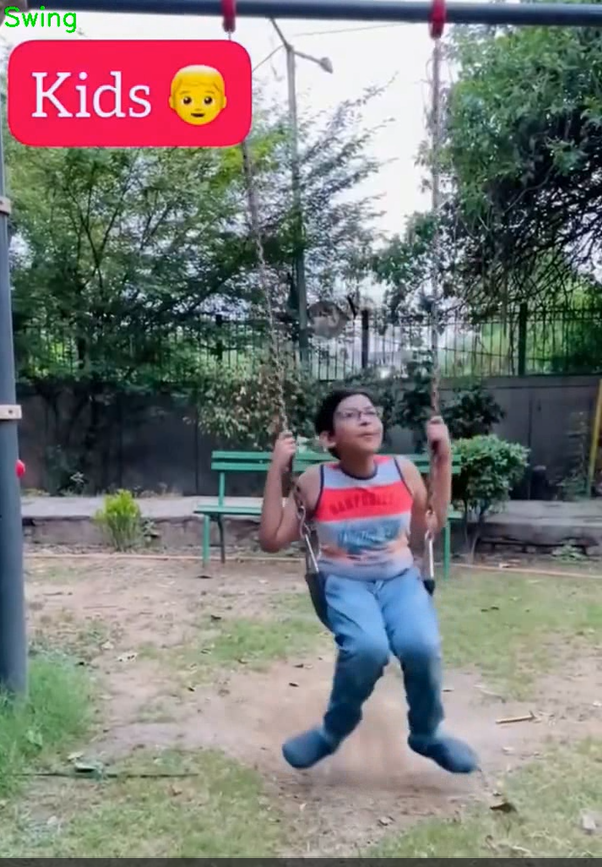
\includegraphics[width=0.5\textwidth]{Figures/swing_lrcn.png}
        \begin{figure}[h!]
    	\centering
    	
    	\caption[Swing output .]{Swing output.}
    	\label{swing_lrcn.png} 
        \end{figure}
        
    \item HorseRace

        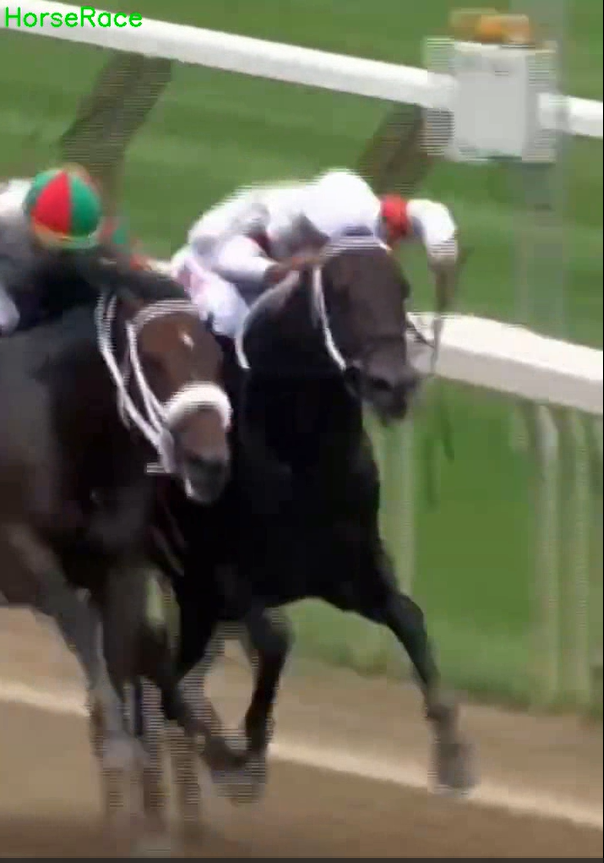
\includegraphics[width=0.5\textwidth]{Figures/race_lrcn.png}
        \begin{figure}[h!]
    	\centering
    	
    	\caption[HorseRace output .]{HorseRace output.}
    	\label{race_lrcn.png} 
        \end{figure}

    \item PlayingPiano

        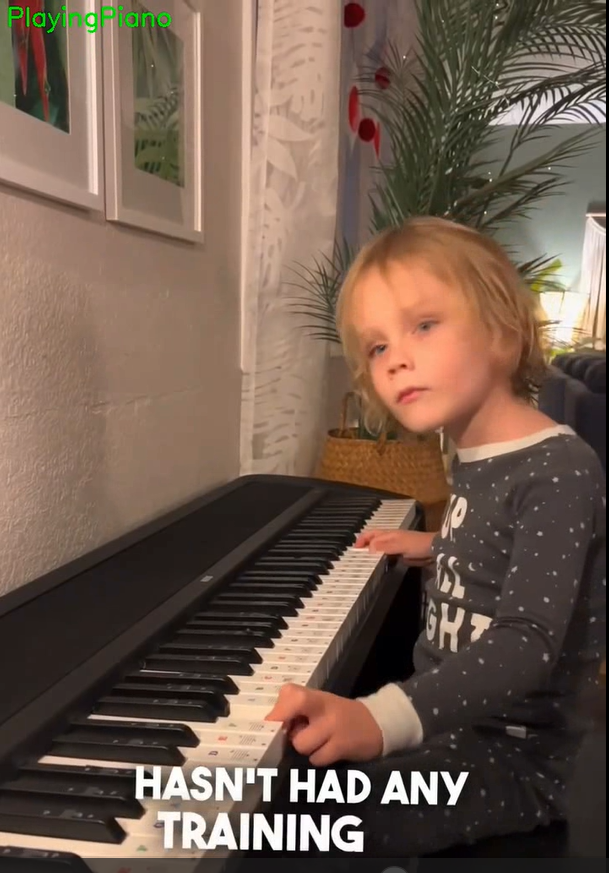
\includegraphics[width=0.5\textwidth]{Figures/piano_lrcn.png}
        \begin{figure}[h!]
    	\centering
    	
    	\caption[PlayingPiano output .]{PlayingPiano output.}
    	\label{piano_lrcn.png} 
        \end{figure}

    \item PushUps

        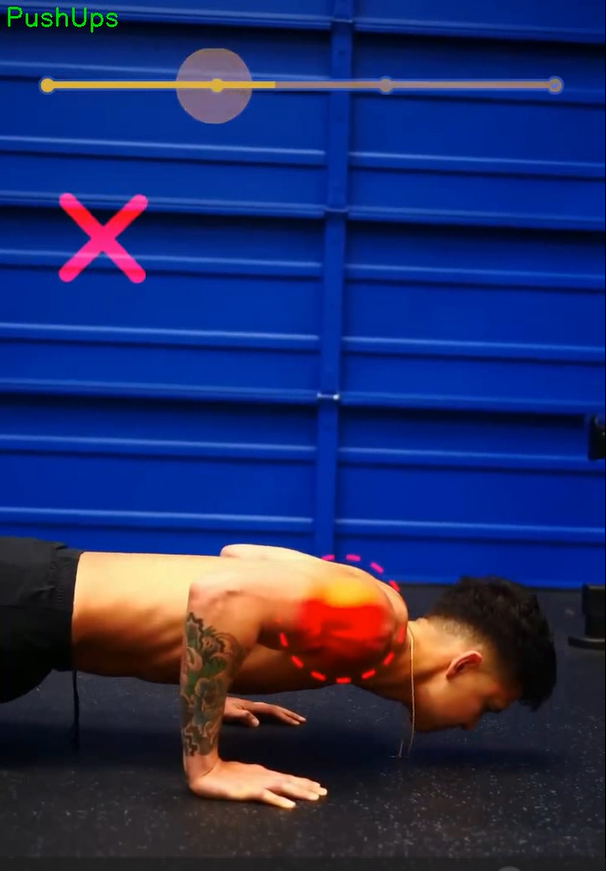
\includegraphics[width=0.5\textwidth]{Figures/pushup_lrcn.png}
        \begin{figure}[h!]
    	\centering
    	
    	\caption[PushUps output .]{PushUps output.}
    	\label{pushup_lrcn.png} 
        \end{figure}
        
    \item Skijet

        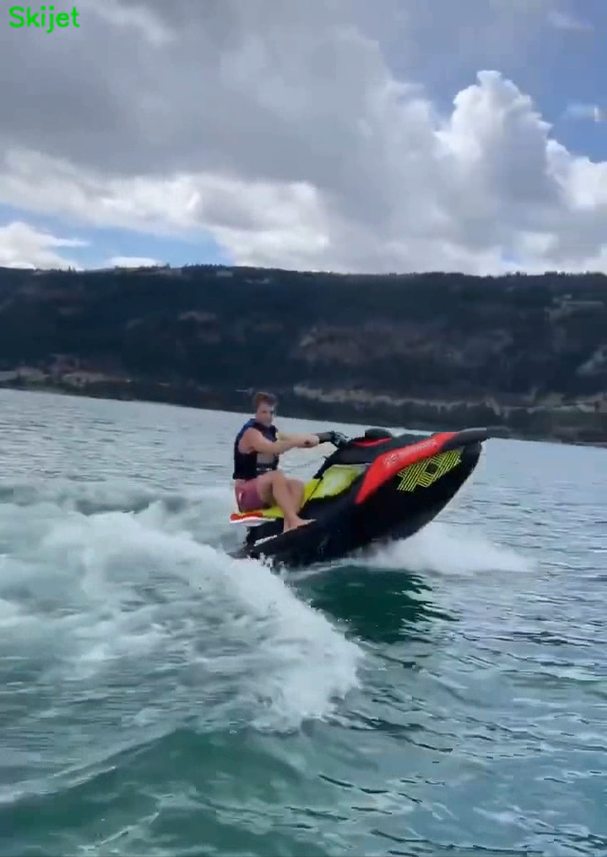
\includegraphics[width=0.5\textwidth]{Figures/skijet_lrcn.png}
        \begin{figure}[h!]
    	\centering
    	
    	\caption[Skijet output .]{Skijet output.}
    	\label{skijet_lrcn.png} 
        \end{figure}

    \item Drumming

        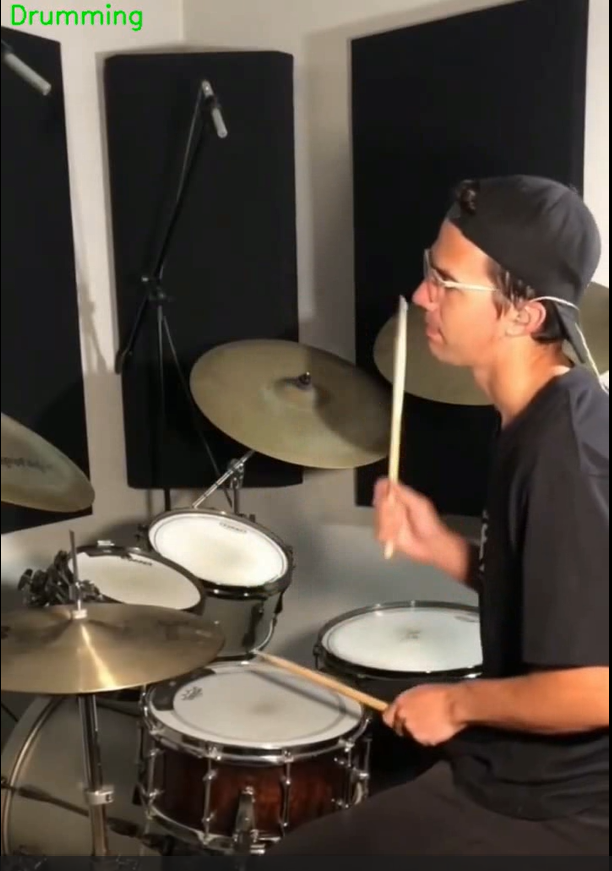
\includegraphics[width=0.5\textwidth]{Figures/drum_lrcn.png}
        \begin{figure}[h!]
    	\centering
    	
    	\caption[Drumming output .]{Drumming output.}
    	\label{drum_lrcn.png} 
        \end{figure}
    
\end{itemize}



\section{Đánh giá các phương pháp}

Trong dự án này ,nhóm đã tiếp cận bài toán theo 3 phương pháp tùy thuộc vào độ phức tạp , độ chính xác cần thiết và khả năng tính toán.Đối với phương pháp sử dụng thư viện mediapipe kết hợp với LSTM phù hợp với các bài toán đơn giản , nhận diện ít hành động.Đối với nhận diện hành động qua video , Nhóm nhận thấy phương pháp xây dựng model LRCN cho ra kết quả nhận diện hành động từ video tốt hơn phương pháp sử dụng ConvLSTM . Tuy nhiên tùy thuộc vào từng bài toán mà chúng ta chọn phương pháp sao cho hiệu quả nhất . 

\begin{itemize}
    \item Model ConvLSTM sử dụng các lớp ConvLSTM2D để học các đặc trưng tĩnh và động từ các khung hình video cùng một lúc.
    \item Model LRCN sử dụng các lớp TimeDistributed(Conv2D) để trích xuất các đặc trưng tĩnh từ từng khung hình riêng lẻ, sau đó mới đưa các đặc trưng này vào một lớp LSTM để học các mối quan hệ động giữa các khung hình.
\end{itemize}
\subsection{Cách tiếp cận sử dụng ConvLSTM2D}
- Các lớp ConvLSTM2D trích xuất các đặc trưng không gian thời gian đồng thời duy trì mối quan hệ không gian.
- Học các đặc trưng không gian và thời gian đồng thời bằng cách tích hợp các phép toán tích chập trực tiếp vào các lớp LSTM.
- Các phép toán tích chập được sử dụng để trích xuất đặc trưng không gian từ các khung hình, trong khi các cổng LSTM được sử dụng để học các mối quan hệ thời gian giữa các khung hình.
- Độ phức tạp của video: ConvLSTM có thể phù hợp hơn cho các video có các hành động phức tạp hoặc dài.
- Độ chính xác cần thiết: ConvLSTM có thể đạt được độ chính xác cao hơn trong một số trường hợp.
- Khả năng tính toán: ConvLSTM thường đòi hỏi nhiều tài nguyên tính toán hơn so với LRCN.
\subsection{Cách tiếp cận sử dụng LRCN}

- LRCN kết hợp các lớp CNN và LSTM trong cùng một mô hình.
- Các lớp CNN được sử dụng để trích xuất các đặc trưng không gian từ các frames.
- Các đặc trưng không gian được đưa vào các lớp LSTM tại mỗi bước thời gian để mô hình hóa chuỗi thời gian.
- Cách tiếp cận này cho phép mô hình học trực tiếp các đặc trưng không gian thời gian trong quá trình huấn luyện end-to-end, dẫn đến một mô hình mạnh mẽ hơn.
- Trong LRCN, lớp TimeDistributed được sử dụng để áp dụng cùng một lớp cho mọi khung hình của video một cách độc lập.
- Lớp TimeDistributed cho phép model LRCN xử lý toàn bộ video trong một lần, thay vì phải xử lý từng khung hình riêng lẻ.

Ưu điểm của LRCN:
\begin{itemize}
    \item Có thể học các đặc trưng không gian thời gian trực tiếp từ dữ liệu .
    \item Có thể nắm bắt các mối quan hệ dài hạn giữa các frames trong một sequence .
    \item Có thể huấn luyện end-to-end, đơn giản hóa quá trình huấn luyện .
\end{itemize}

Nhược điểm của LRCN:

\begin{itemize}
    \item Có thể khó huấn luyện hơn so với cách tiếp cận sử dụng CNN và LSTM riêng biệt.
    \item Có thể gặp khó khăn trong việc nắm bắt các mối quan hệ phức tạp giữa các đặc trưng không gian và thời gian.
\end{itemize}


Khi nào nên chọn LRCN:
\begin{itemize}
    \item Khi cần nắm bắt các mối quan hệ dài hạn giữa các frames trong một sequence.
    \item Khi cần một mô hình mạnh mẽ có thể học các đặc trưng không gian thời gian trực tiếp từ dữ liệu.
\end{itemize}



\section{Hướng phát triển trong tương lai}

\begin{itemize}
	\item Trong tương lai, nhóm muốn tạo ra một app trên điện thoại để có thể đến được gần hơn với nhiều người. 
	
	\item Muốn phát triển lên thành sản phẩm hoàn chỉnh có tính thực tế cao hơn.	
	
	\item Cải thiện model tốt hơn , dự đoán chính xác hơn , nhanh hơn . 
\end{itemize}



